\section{Architecture}
When the project case was presented to the group it was discussed what
subsystems the MES should consist of. It was clear from the start that an OPC-UA
client was needed, as this should connect to the beer production machine. This
client should in some way store the collected data from the production machine,
which means that some kind of database should be a part of the MES. As the data
would only consist of simple data types, integers, strings, etc., it was decided
to use a relational database. This way, data from different batches could easily
be stored in such a way that the relations between the data could be kept as
needed. By having a database, the subsystems do not have to store data
locally, thus making the same data available for other parts of the system,
securing data consistency. \\

It was discussed whether to develop a desktop client functioning as a dashboard
to control the production machine, or if it should be a web client. The decision
landed on a web client. A web client is a more simple solution for the dashboard
as it can run in all supported web browsers. If the company then chooses to
change hardware, the dashboard is still functional. \\
 

To make the data from the database available to all subsystems in the MES, 
it was decided to develop a REST API. The REST API acts as a translator
between the subsystems in the MES, therefore simplifying the data management.
An example could be that the dashboard needs the data for a specific batch to
generate a batch report. Instead of having the dashboard communicate directly
with the database, a layer is added, the REST API, which both adds security and
handles the queries in a uniform way. The database then sends a query result to
the REST API which then translates the SQL to JSON for the dashboard to read
and display to the user. \\

An overview of the MES to be developed can seen in figure
\ref{figure:architucture_diagram}.

\begin{figure}[ht]
	\centering 
	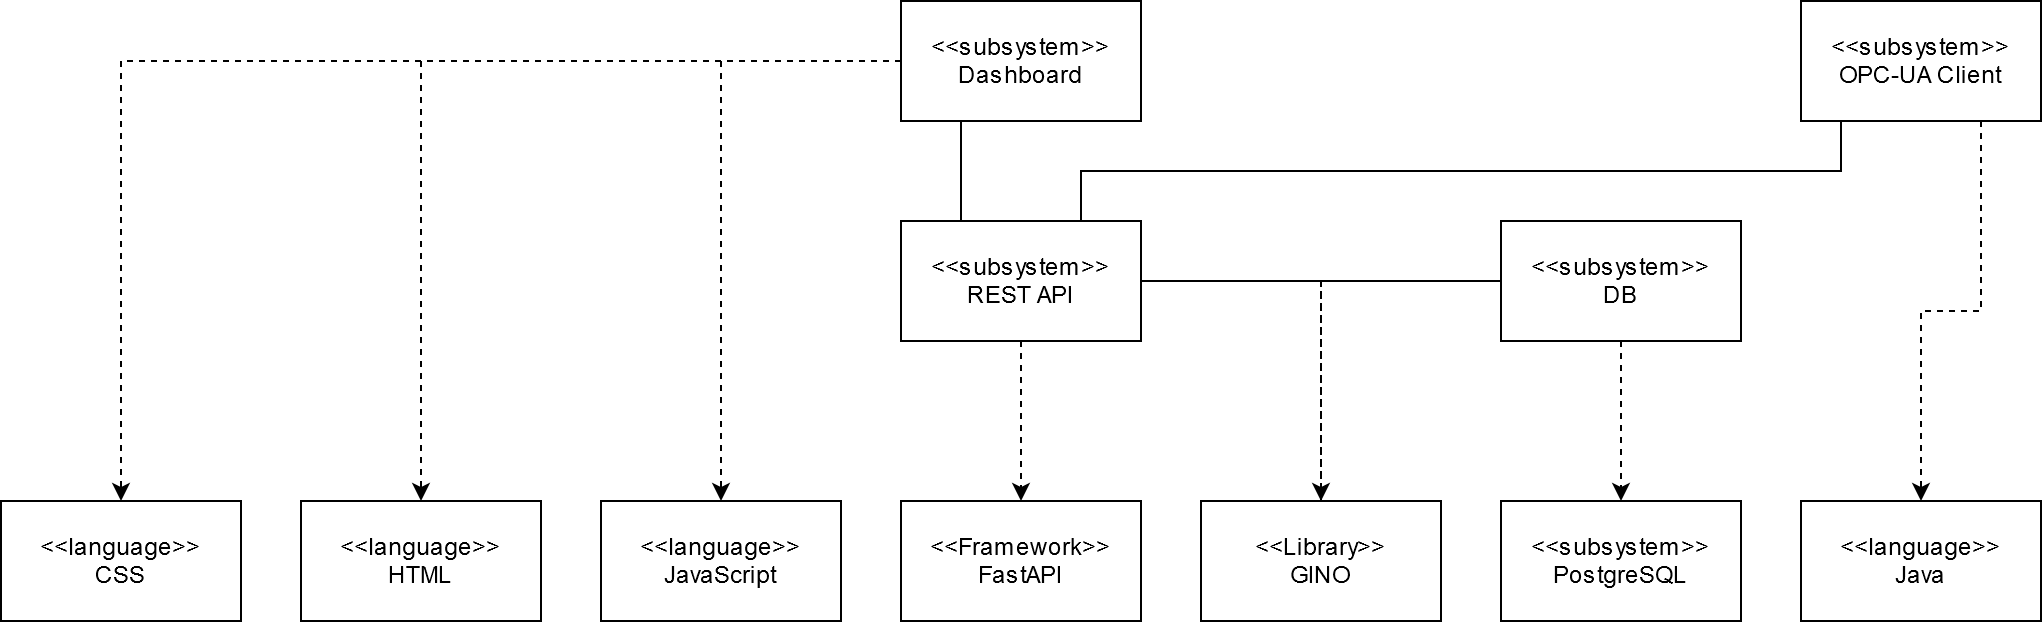
\includegraphics[scale=0.24]{images/diagrams/architecture_diagram.png}
	\caption{Software Architecture Diagram}
	\label{figure:architucture_diagram} 
\end{figure}
